\chapter{Conception}

Au vu de nos besoins et de nos choix de solutions scientifiques, nous avons mis en place une architecture de type
\textbf{client-serveur} dont :
\begin{itemize}
    \item le client est une application mobile qui gère les interactions avec l'utilisateur ainsi que la géolocalisation
    ; les actes de dialogue de l'utilisateur sont transmis au serveur afin d'obtenir la réponse de l'agent ;
    \item le serveur gère la logique de l'agent conversationnel et communique ses réponses au client.
\end{itemize}

~\\\indent
Dans cette partie nous aborderons les différents diagrammes \texttt{UML} permettant de modéliser cette solution.


\section{Cas d'utilisation}

La figure \ref{usecase-diagram} détaille le cas d'utilisation de l'application : "Programmer une alarme".

\begin{figure}[!h]
    \centering
    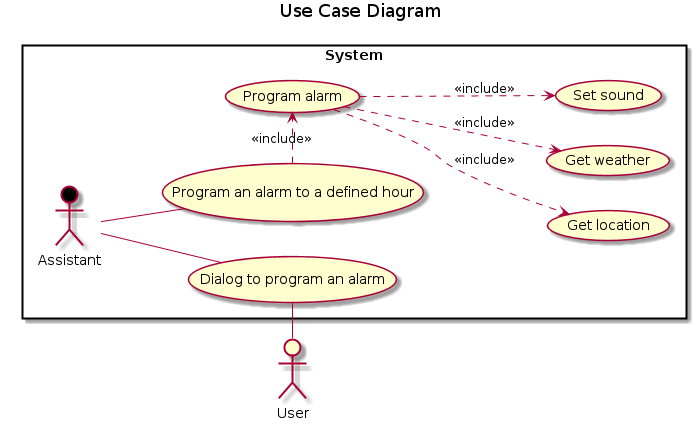
\includegraphics[width=\textwidth]{../docs/conception/build/usecaseDiagram.png}
    \caption{Diagramme de cas d'utilisation}
    \label{usecase-diagram}
\end{figure}


\section{Activités}

De même, la figure \ref{activity-diagram} explicite la logique de l'exécution du cas d'utilisation principal.

\begin{figure}[!h]
    \centering
    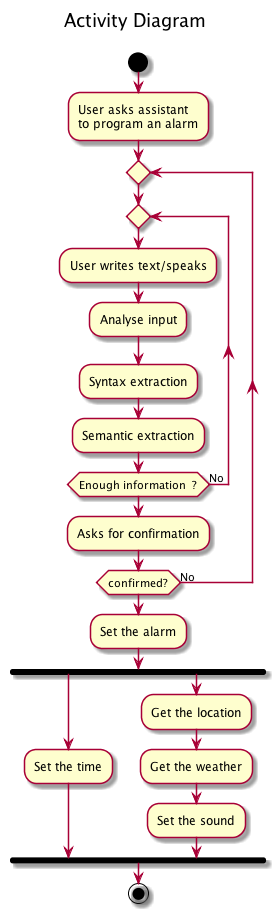
\includegraphics[width=0.4\textwidth]{../docs/conception/build/activityDiagram.png}
    \caption{Diagramme d'activité}
    \label{activity-diagram}
\end{figure}


\section{Classes}

Pour mettre en œuvre ce cas d'utilisation, les figures \ref{class-diagram-client} et \ref{class-diagram-server}
illustrent la modélisation par classes (respectivement côté client et côté serveur) de la solution.

\begin{figure}[!h]
    \centering
    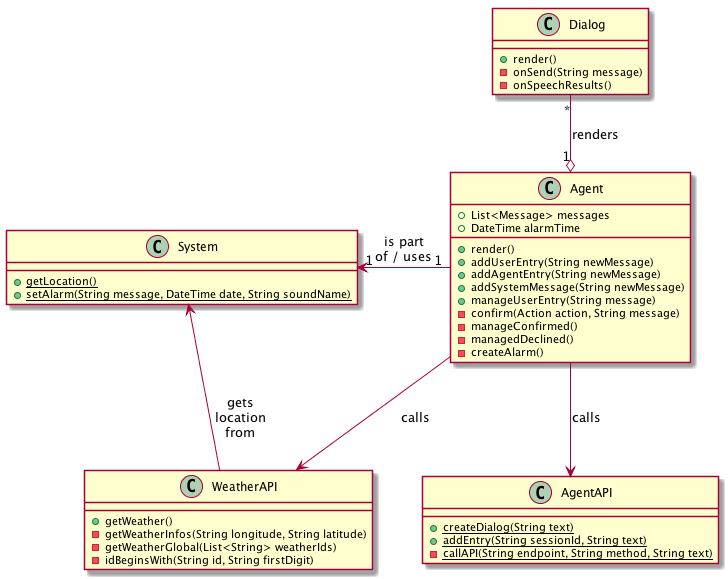
\includegraphics[width=1.1\textwidth,center]{../docs/conception/build/classDiagram_Client.png}
    \caption{Diagramme de classes côté client}
    \label{class-diagram-client}
\end{figure}

\begin{figure}[!h]
    \centering
    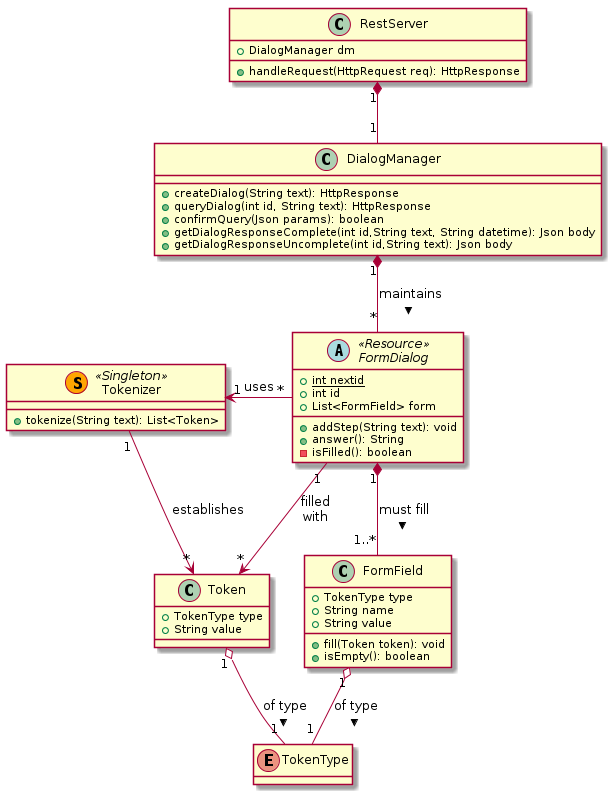
\includegraphics[width=0.9\textwidth]{../docs/conception/build/classDiagram_Server.png}
    \caption{Diagramme de classes côté serveur}
    \label{class-diagram-server}
\end{figure}


\section{Packages}

La figure \ref{package-diagram} précise le découpage des classes choisies en différents packages logiques.

\begin{figure}[!h]
    \centering
    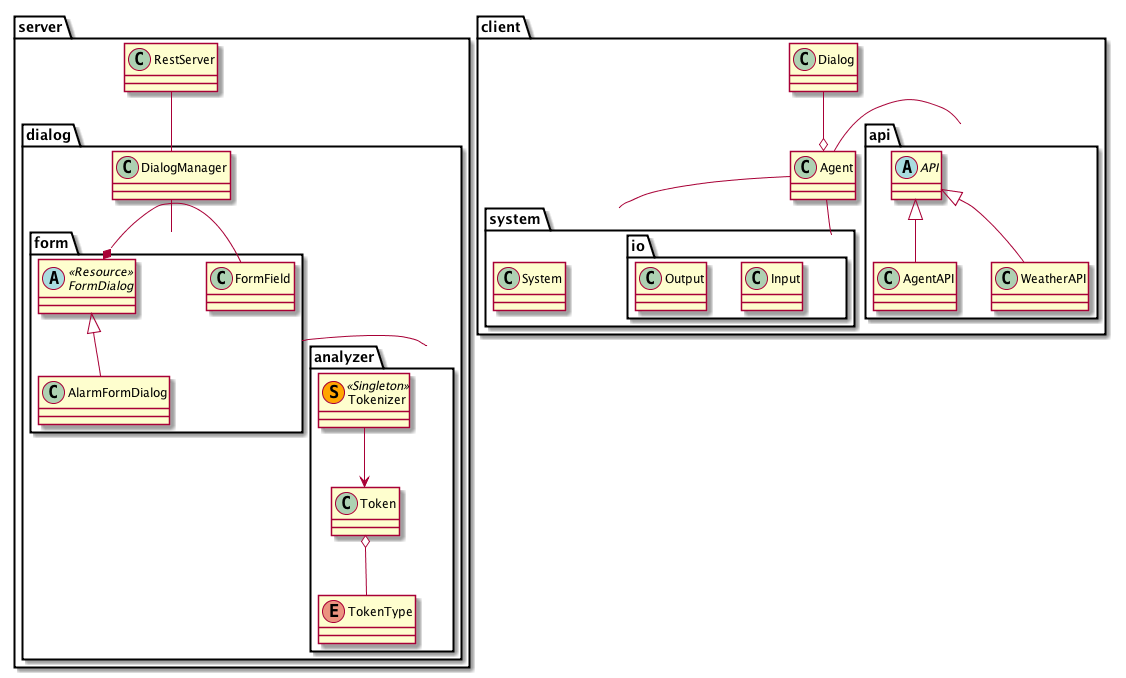
\includegraphics[width=1.1\textwidth,center]{../docs/conception/build/packageDiagram.png}
    \caption{Diagramme de packages}
    \label{package-diagram}
\end{figure}


\section{Séquences}

Pour terminer, la figure \ref{sequence-diagram} détaille dans un diagramme de séquences la logique du cas d'utilisation :
ce qu'il se passe lorsqu'un utilisateur dialogue avec l'agent.\\
\textit{À noter que ce diagramme est simplifié pour être plus
visuel : il n'illustre pas l'aspect asynchrone de certains traitements.}


\begin{figure}[!h]
    \centering
    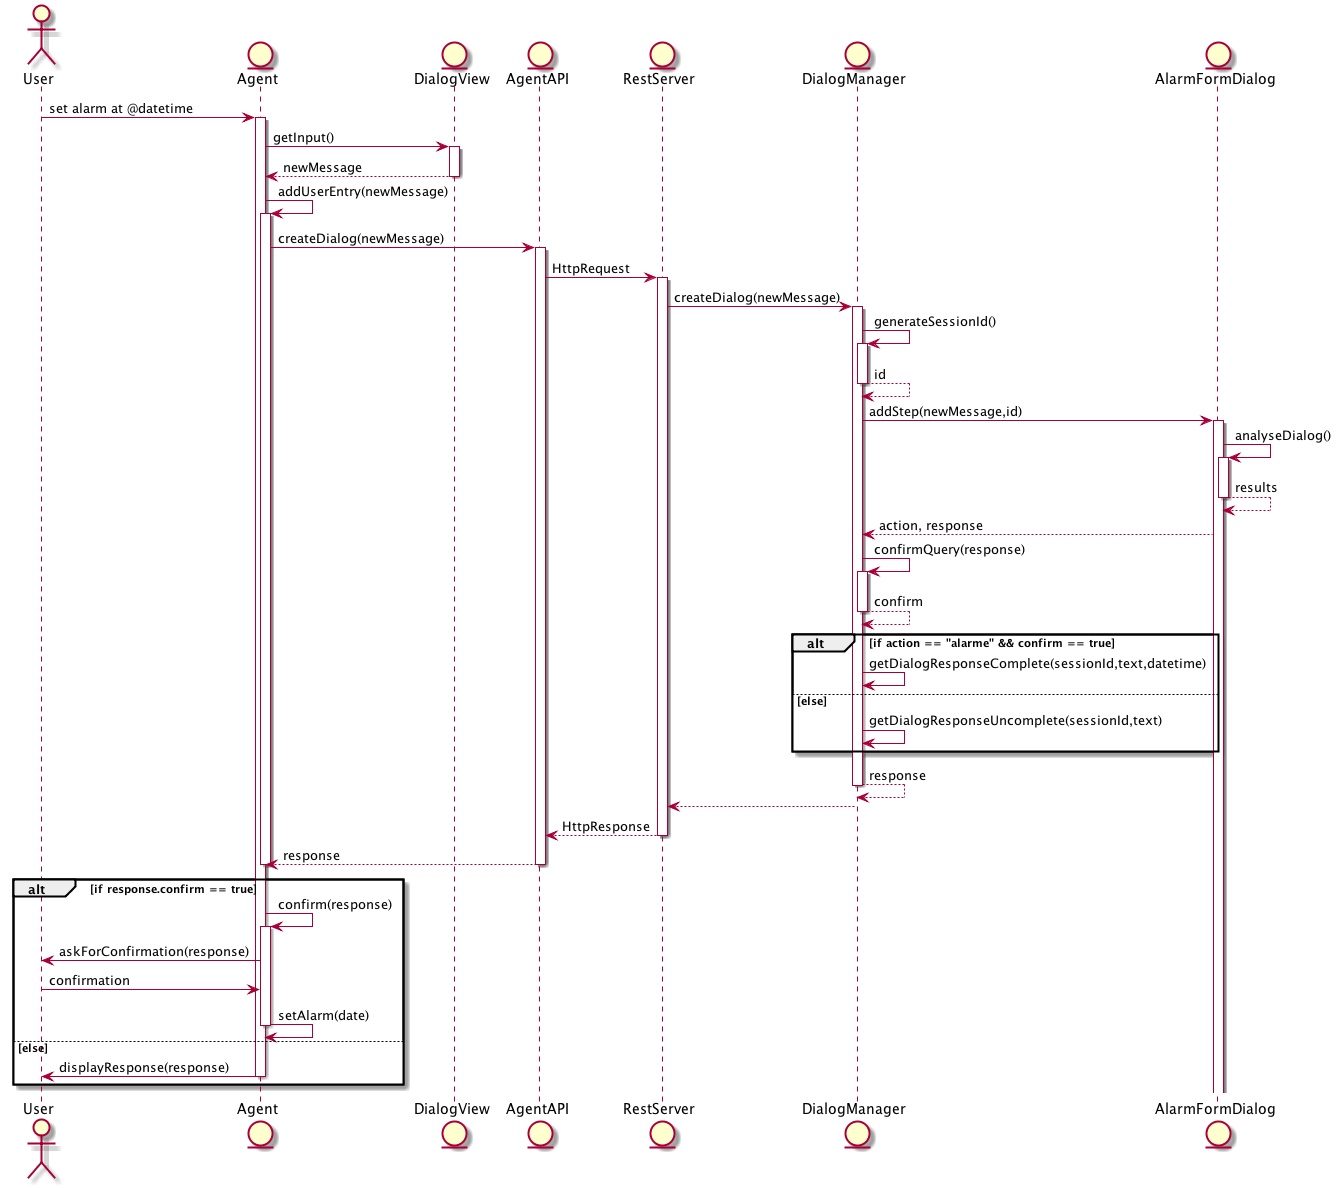
\includegraphics[width=1.3\textwidth,center]{../docs/conception/build/sequenceDiagram.png}
    \caption{Diagramme de séquences}
    \label{sequence-diagram}
\end{figure}
